% begin module vertical-line-test
\begin{frame}
\frametitle{The Vertical Line Test}
Question: How can we tell if a curve is the graph of a function or not? 

Answer: Use the vertical line test.

\begin{proof}[The Vertical Line Test]
A curve is the graph of a function if and only if no vertical line intersects it more than once.
\end{proof}

\begin{tabular}{ccc}
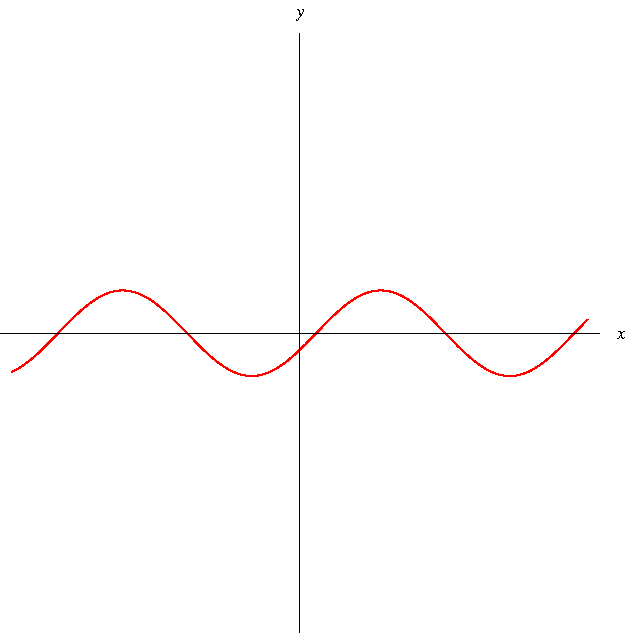
\includegraphics[height=3.8cm]{precalculus/pictures/01-02-vlt3.pdf} &%
\only<handout:0| -2>{%
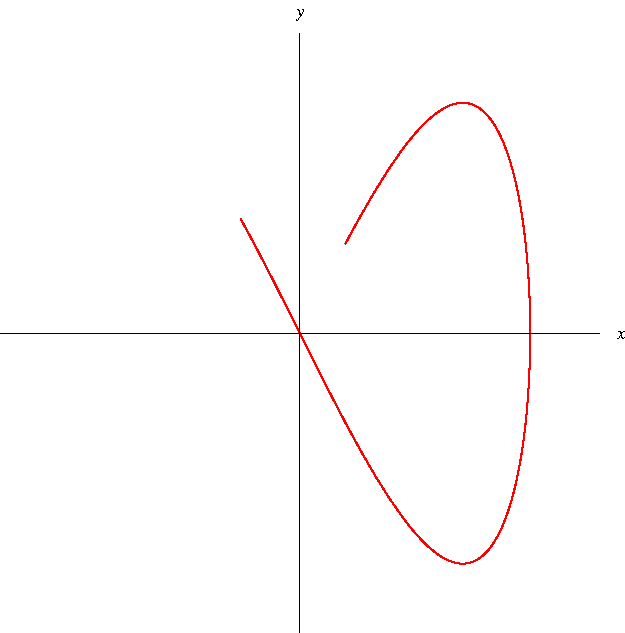
\includegraphics[height=3.8cm]{precalculus/pictures/01-02-vlt1a.pdf}%
}%
\only<handout| 3->{%
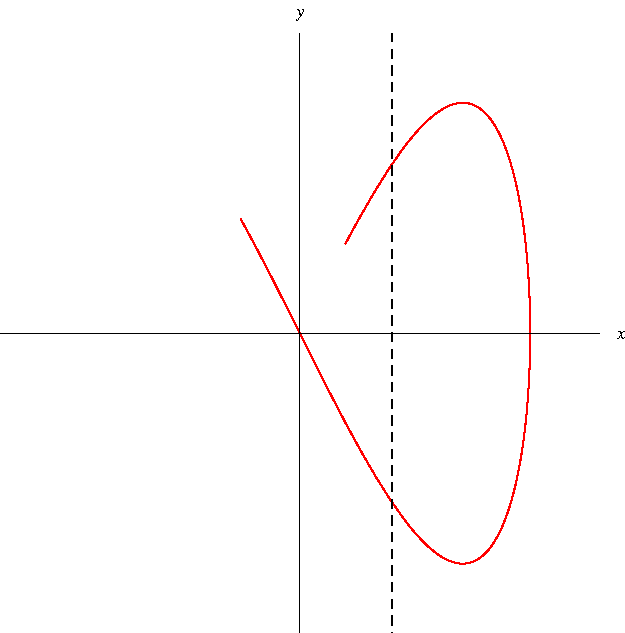
\includegraphics[height=3.8cm]{precalculus/pictures/01-02-vlt1b.pdf}%
} &%
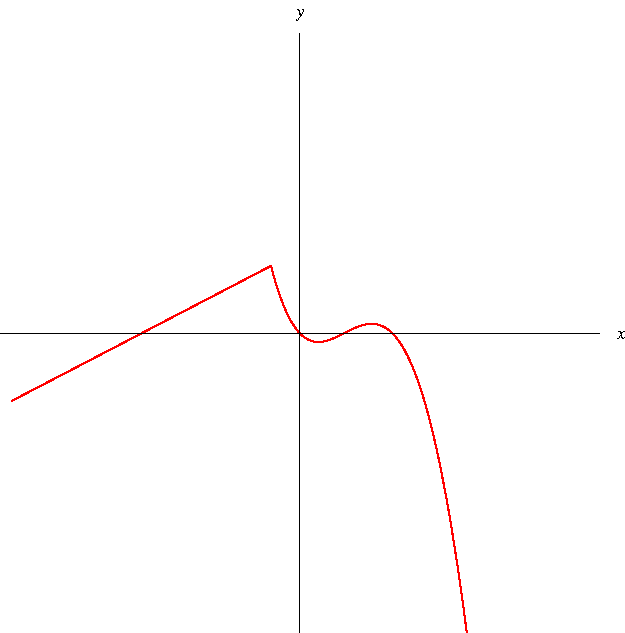
\includegraphics[height=3.8cm]{precalculus/pictures/01-02-vlt2.pdf} \\%
\uncover<2->{\alert<handout:0| 2>{Function}} &
\uncover<3->{\alert<handout:0| 3>{Not a function}} &
\uncover<4->{\alert<handout:0| 4>{Function}}
\end{tabular}
\end{frame}
% end module vertical-line-test
